\documentclass{beamer}

\usepackage{pdfpages}
\usepackage{listings}
\usepackage[scaled=.8]{zi4}

\lstdefinestyle{customSQL}{
    %belowcaptionskip=1\baselineskip,
    breaklines=true,
    frame=lines,
    %xleftmargin=10pt,
    language=SQL,
    showstringspaces=false,
    numbers=left,
    numberstyle=\footnotesize\ttfamily,
    stepnumber=1,
    numbersep=5pt,
    basicstyle=\small\ttfamily,
    keywordstyle=\bfseries\color{blue!40!black},
    commentstyle=\itshape\color{gray!80!black},
    stringstyle=\color{orange},
    morekeywords={
        LOOP,
        replace,
        procedure,
        cursor,
        begin,
        open,
        end,
        close,
        is,
        fetch,
        if,
        declare,
        references,
        exit,
        elsif,
        for,
        each,
        row,
        after
    }
}


%Information to be included in the title page:
\title{Final Project Presentation}
\author{Hanlin He \and Kai Kang}
\institute{University of Texas at Dallas}
\date{\today}



\begin{document}

\frame{\titlepage}

\begin{frame}
\frametitle{EER Diagram}
\centering
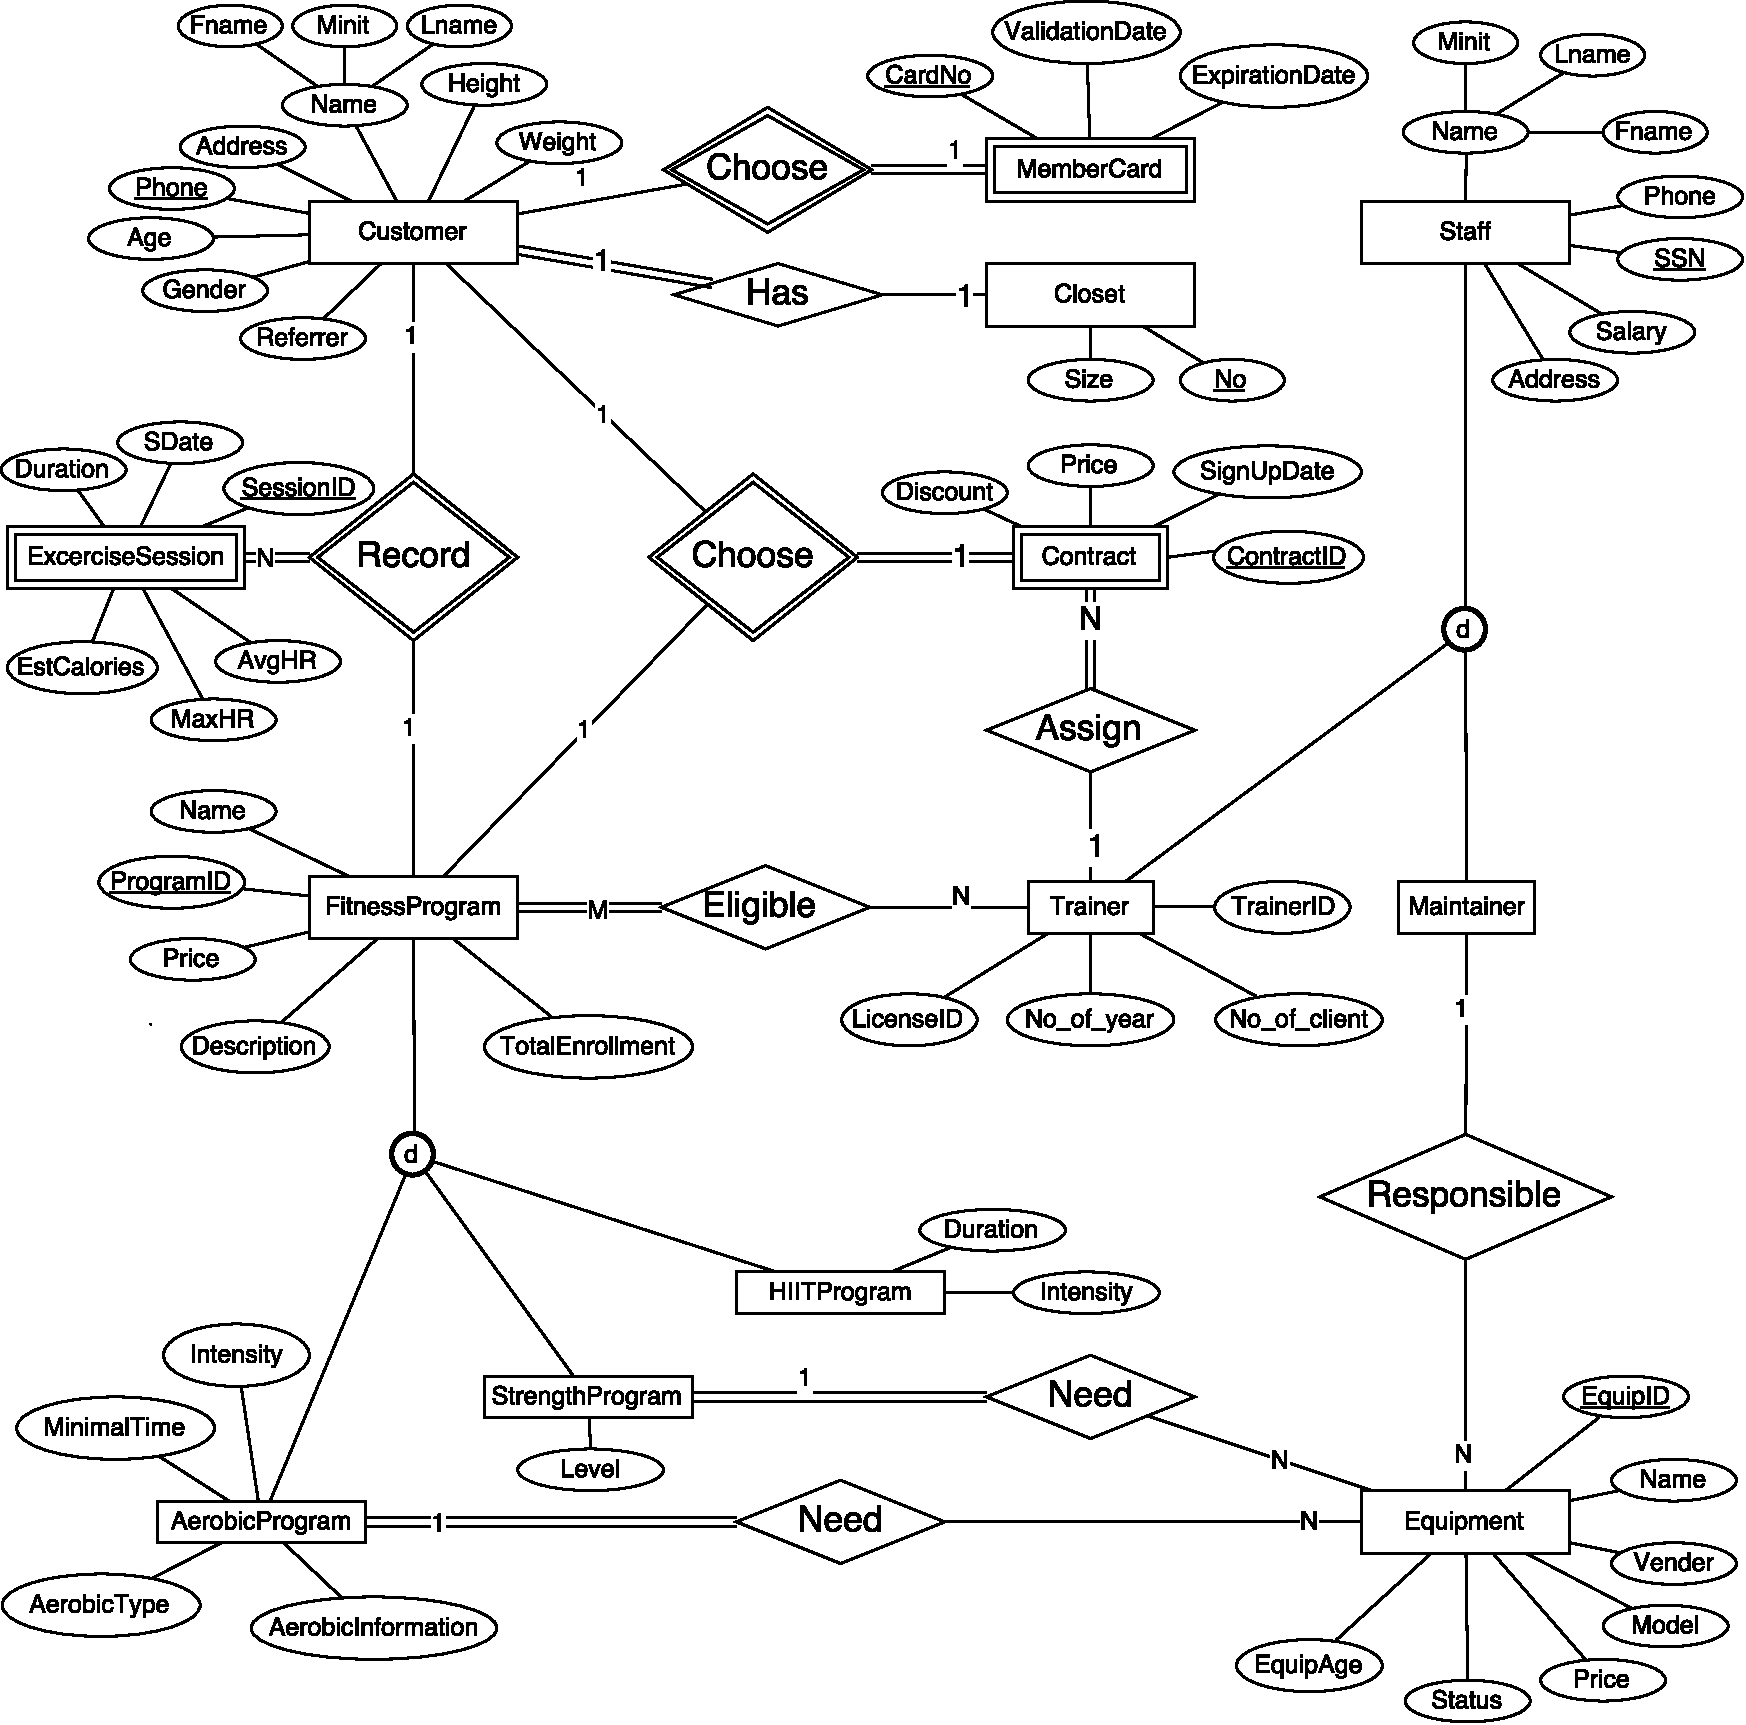
\includegraphics[height=.85\textheight]{img/eer}
\end{frame}

\begin{frame}
\frametitle{Relational Schema after Mapping}
\centering
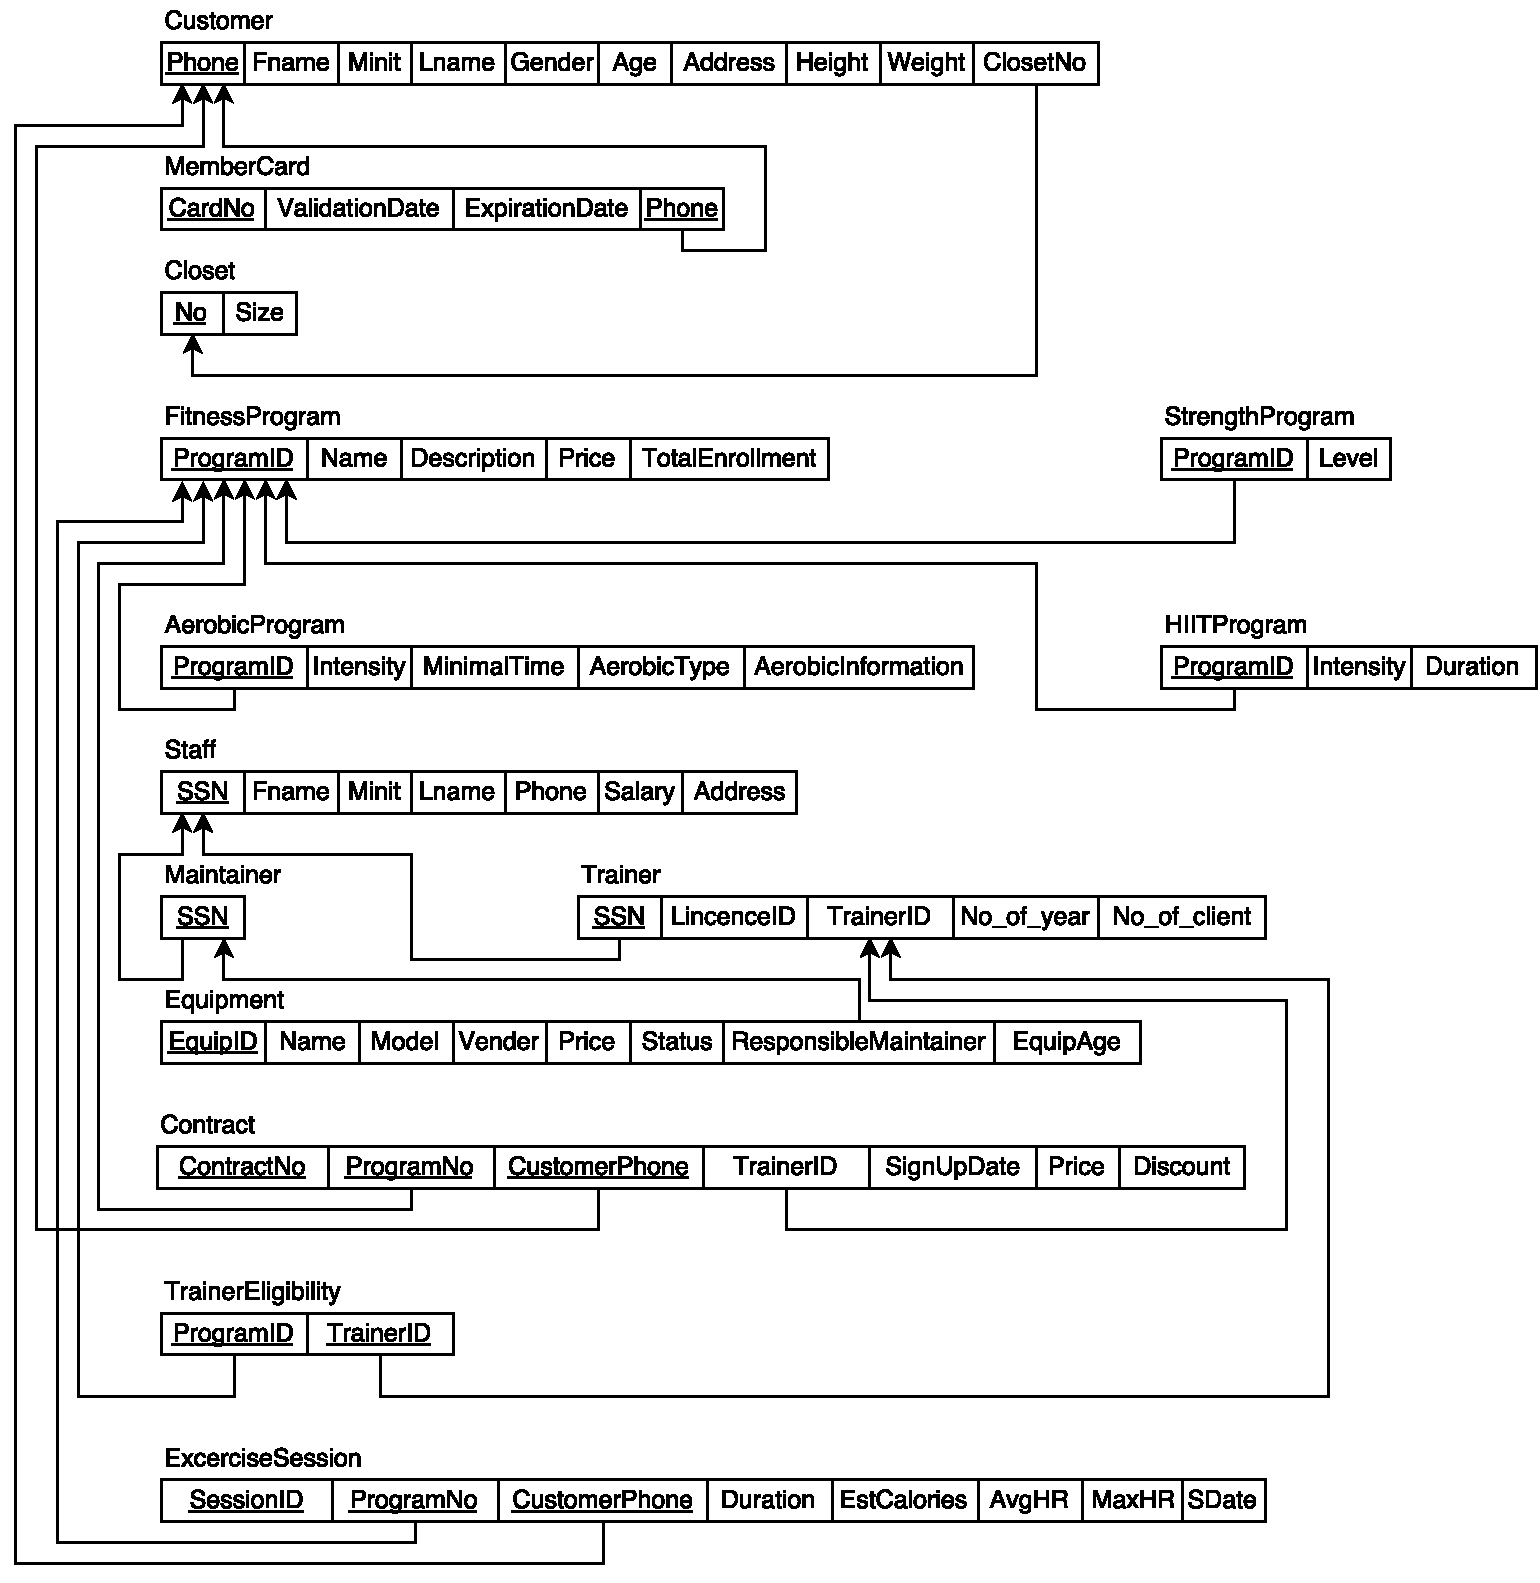
\includegraphics[height=.85\textheight]{img/sdam}
\end{frame}

\begin{frame}
\frametitle{Functional Dependencies}
\centering
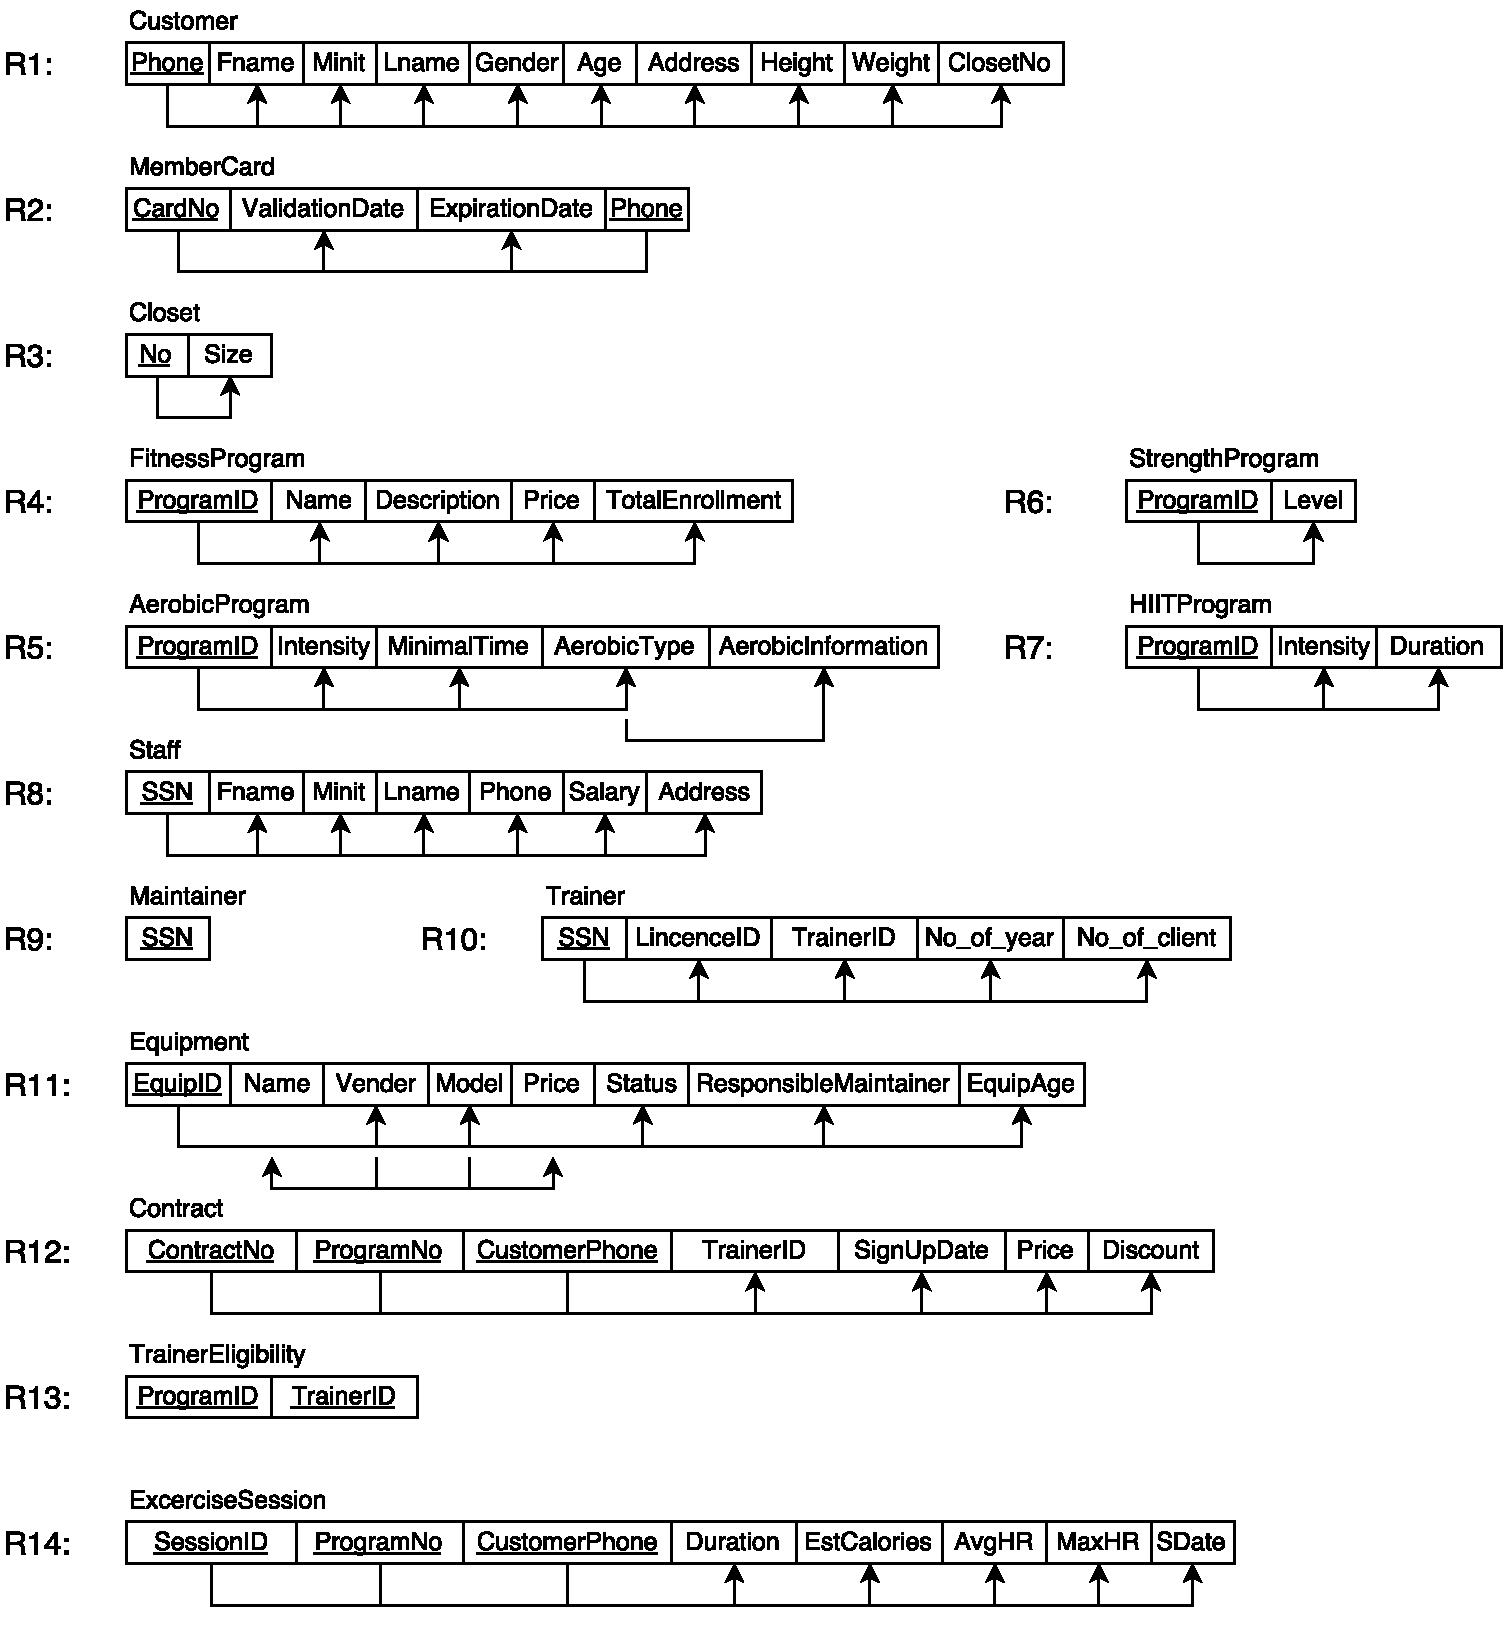
\includegraphics[height=.85\textheight]{img/fd}
\end{frame}

\begin{frame}
\frametitle{Normalization}
\centering
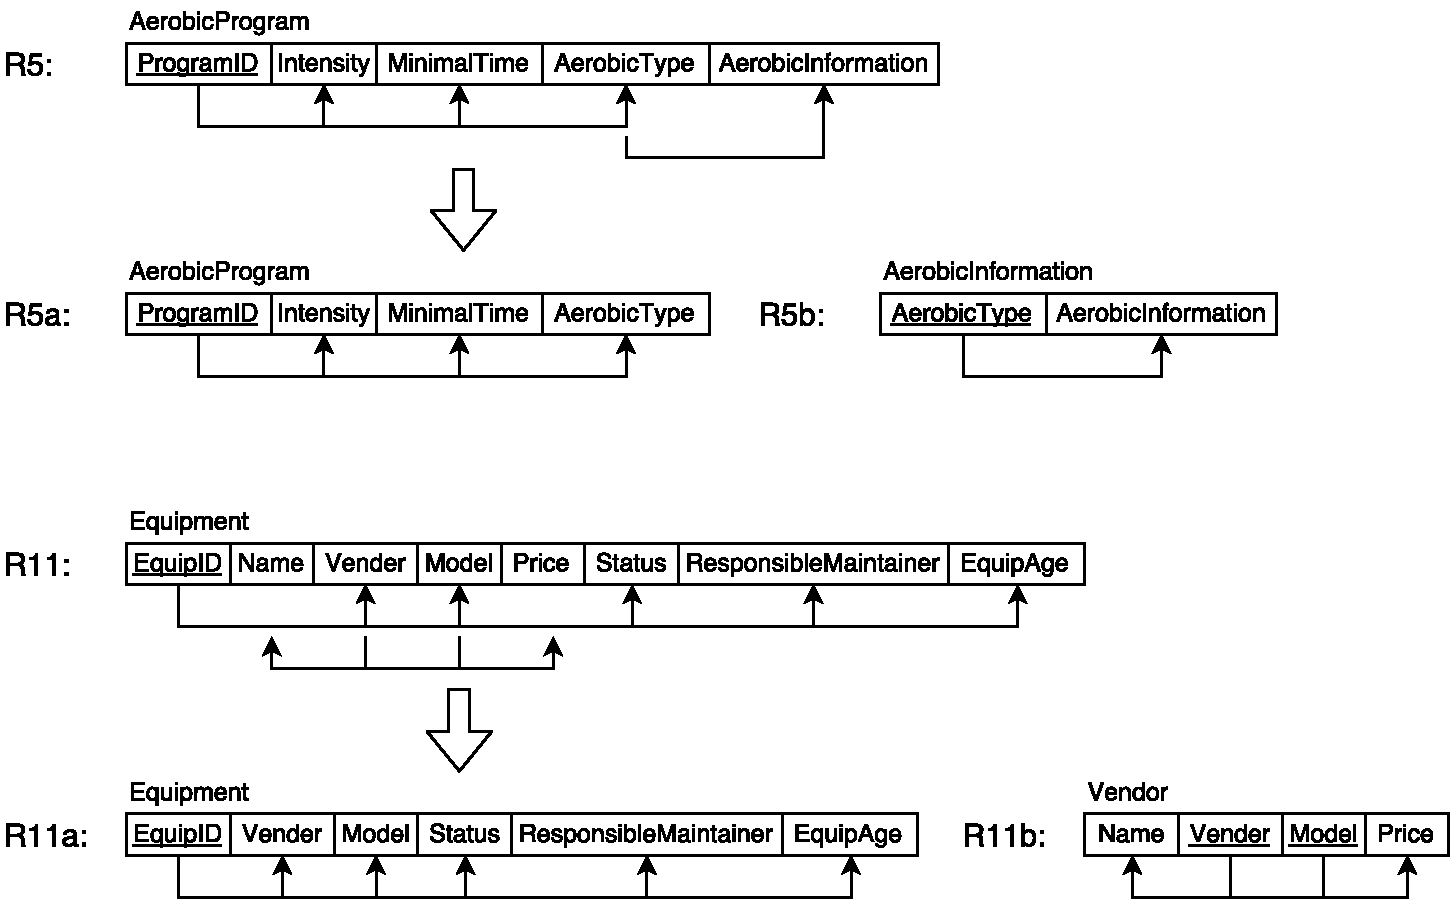
\includegraphics[width=\textwidth]{img/norm}
\end{frame}

\begin{frame}
\frametitle{Update Total Enrollment of Program}
Each time a record was added to the \textsc{Contract} table,
the $TotalEnrollment$ in table \textsc{FitnessProgram} of the particular program should add 1.

The trigger is defined as follow:

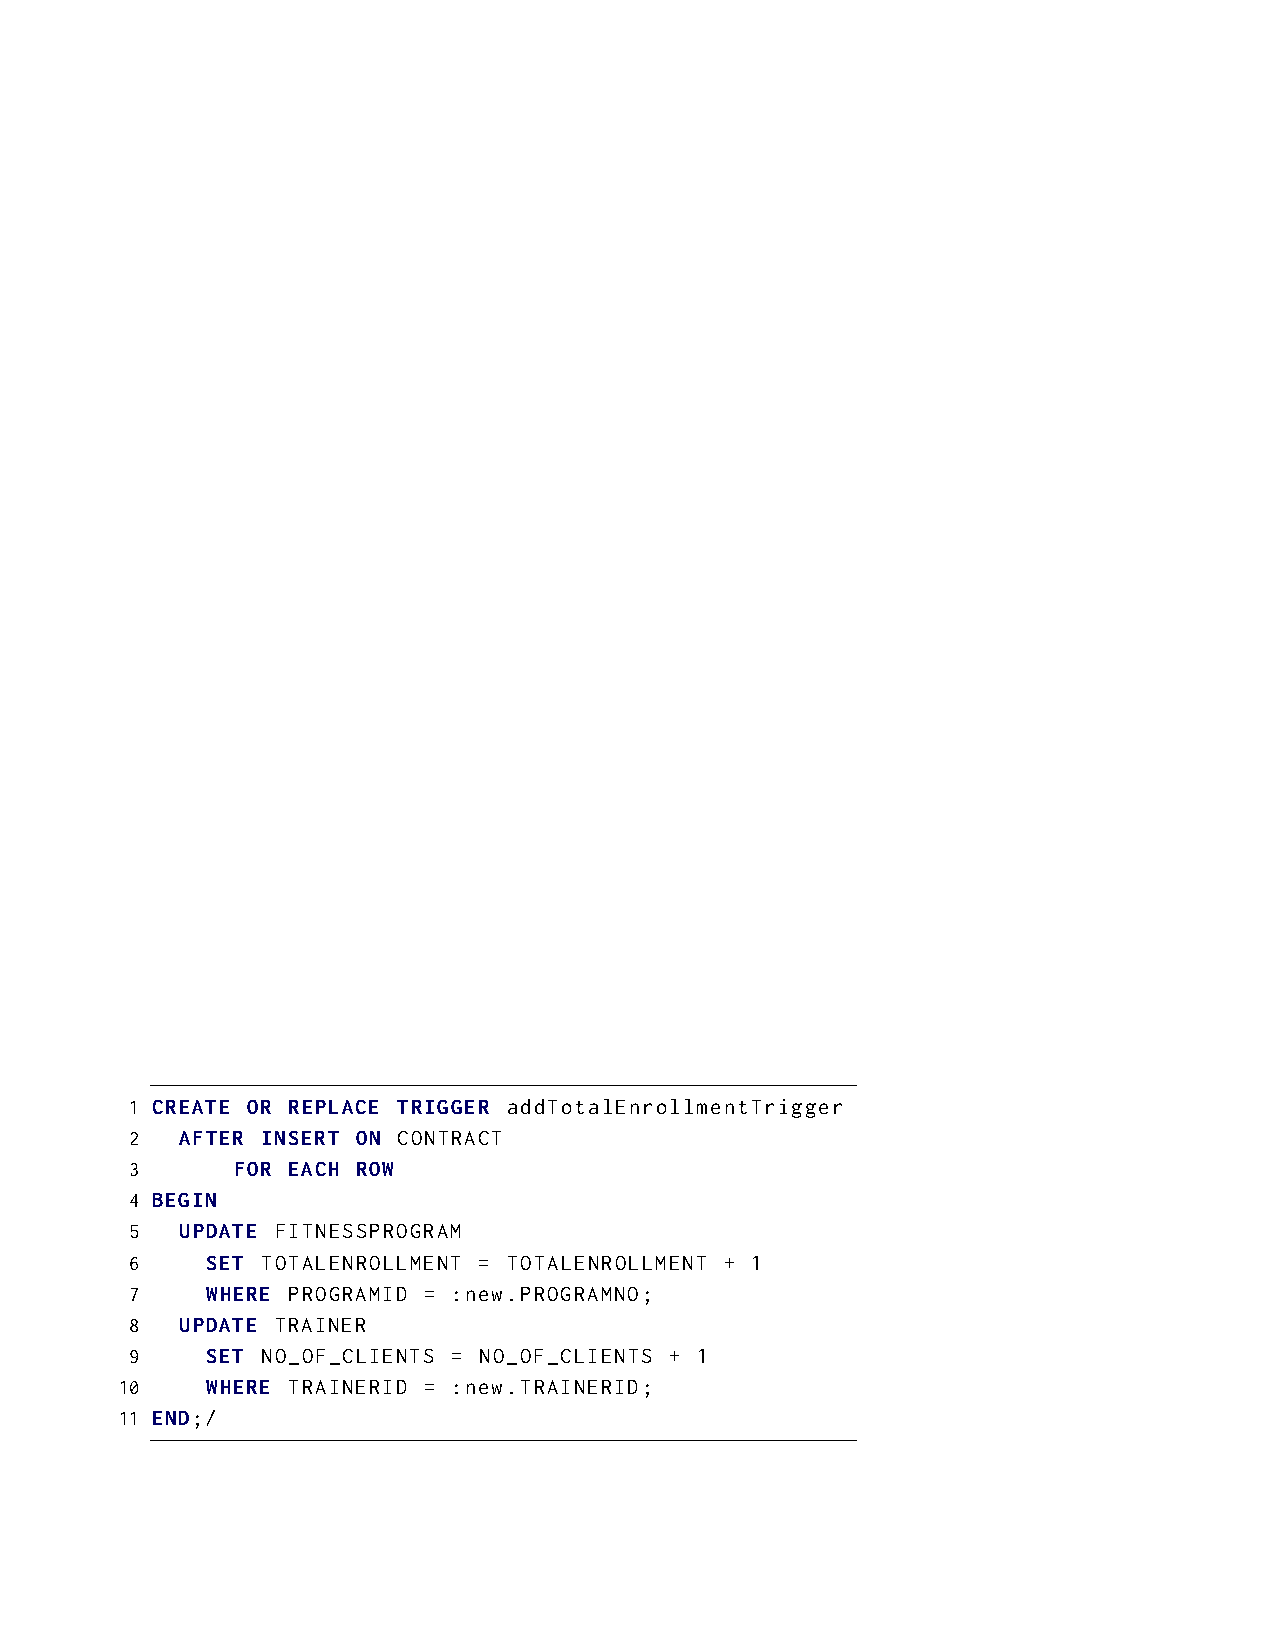
\includegraphics[width=\textwidth]{src/addTotalEnrollmentTrigger}
\end{frame}

\begin{frame}
\frametitle{Trigger: Log All the Changes about Customer}
Each time a record was added/updated/deleted in \textsc{Customer} table,
record the modification in \textsc{Customer\_Log} table.

The trigger is defined as follow:

\centering
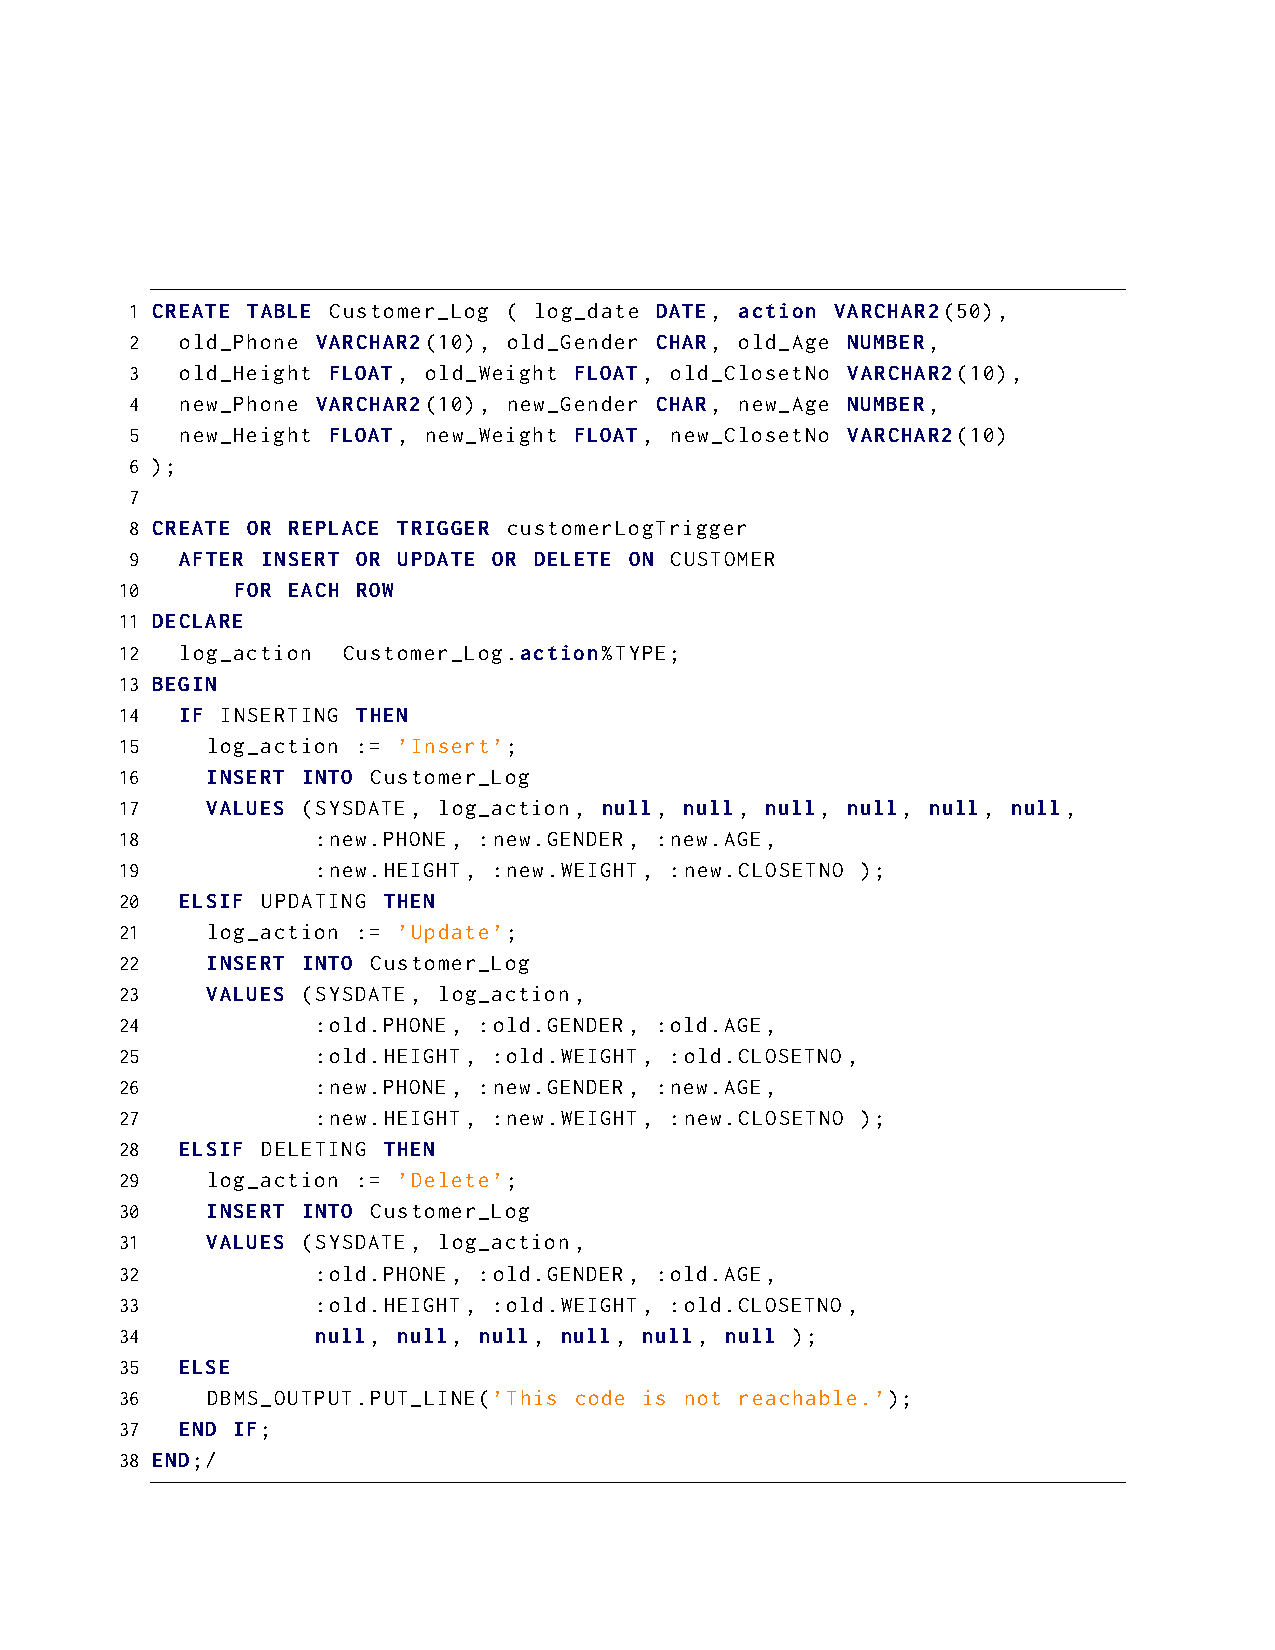
\includegraphics[height=.7\textheight]{src/customerLogTrigger}
\end{frame}

\begin{frame}
    \frametitle{To-do}
\end{frame}

\end{document}
